In this section we present the most important use cases of the eMall. To each use case is associated a corresponding sequence diagram, but we decided to present only the most relevant situations of the use case in the sequence diagrams, so they do not contain all the possible alternatives. We also provide some use cases diagrams in order to better show the relationship between the actors and the actions that they can perform in the system, displaying the features and the capabilities of the application.

\subsection{Unregistered and registered EVD's use cases}
\begin{figure}[H]
    \centering
    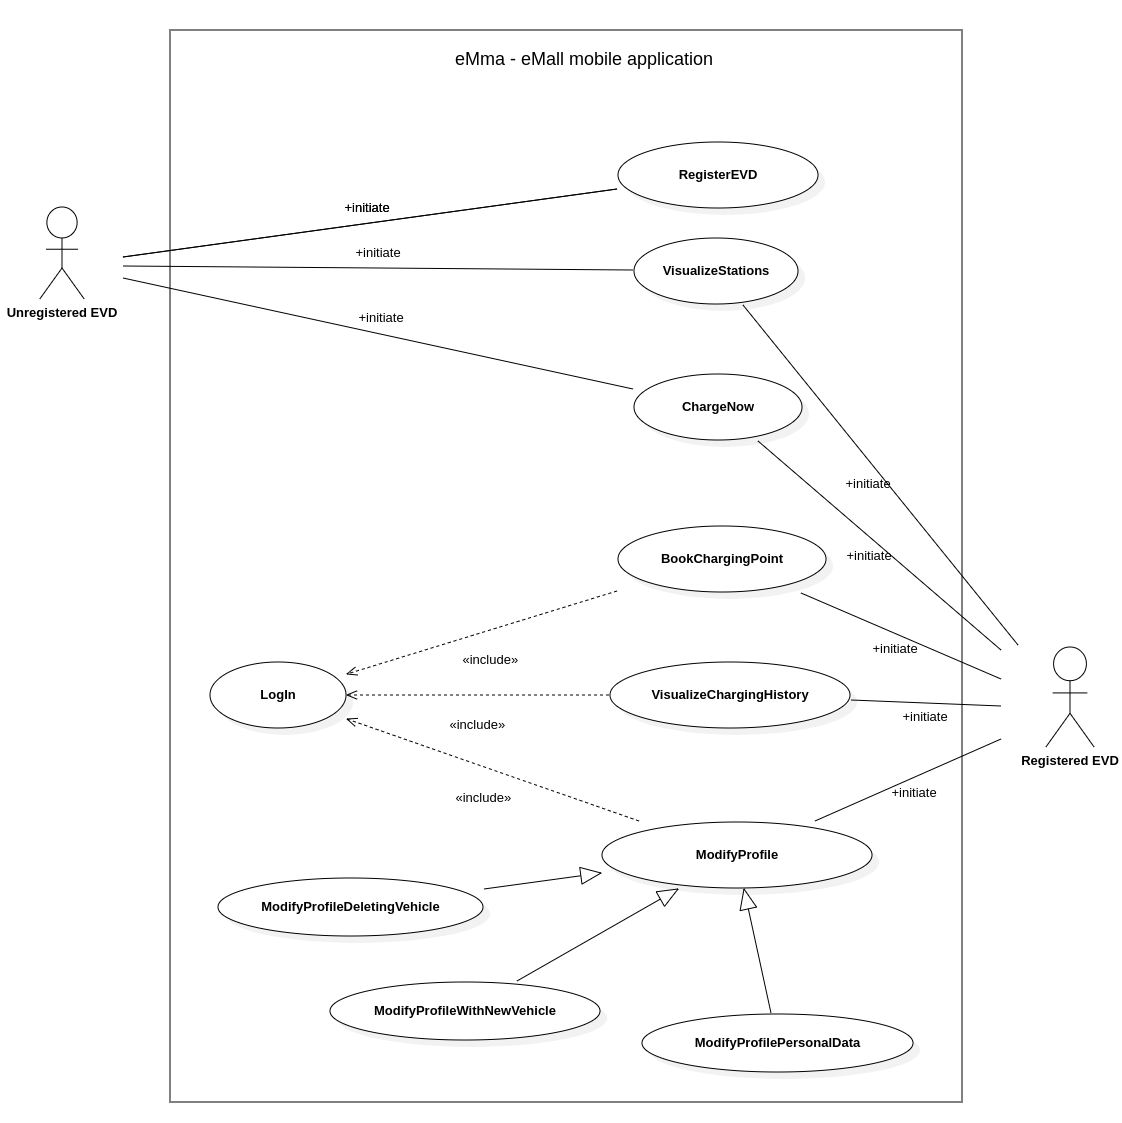
\includegraphics[width=0.9\textwidth, trim = {3cm 2cm 3cm 1cm}, clip]{Images/cp3/UseCaseDiagramEVD.png}
    \caption{Use cases diagram of the registered and unregistered EVD}
\end{figure}

\paragraph{User registration}
\begin{center}
    \begin{longtable}{p{4cm} p{11cm}}
    \multicolumn{2}{r}{\itshape{continue on the next page}}\\
    \endfoot
    \\
    \endlastfoot
    \hline
     Use case name &  RegisterEVD\\
     \hline
     Actor & Unregistered EVD \\
     \hline
     Entry condition & True \\
     \hline
     Event flow & 
         1. User opens the eMma mobile application \newline
         2. User starts the registering process \newline
         3. Users enters his personal data: name, surname, email \newline
         4. System check if the email is in the correct format \newline
         5. User creates a new password and confirms it a second time \newline
         6. System checks the security property of the password \newline
         7. System verifies the ownership of the email \newline
         8. System asks the user for the consent to use his geographical location \newline
         9. User agrees \newline
         10. System asks the user to agree to terms of service \newline
         11. User agrees \newline
         12. <<include>> "ModifyProfileWithNewVehicle" from step 6 \newline
         13. The system asks the user to insert the payment details \newline
         14. The user inserts the payment details \newline
         15. The system checks the correctness of the inserted data \newline
         16. System creates new account and logs in the user\\
     \hline
     Exit condition &  A valid account is created and the system logs in the user \\
     \hline
     Exceptions &  
        a. If the email confirmation process fails eMma shows an error and asks for a new email\newline
        b. If the inserted password doesn't respect security requirements eMma will ask the user for a new password \newline
        c. If the user doesn't confirm the ownership of the email the registration process halts and after 10 minutes the system deletes user's details \newline
        d. If the user doesn't agree to the term of service the registration process halts and after 10 minutes the system deletes user's details \newline
        e. If at any time the user wants to exits the form, the application allows it, but all the data inserted so far are lost if the operation is not completed \\
     \hline
     Special requirements &  Every time the user agrees, a new page is loaded in less than 2 seconds, in order for the application to be perceived as fast \\
     \hline
    \caption{RegisterEVD}
    \label{tab:RegisterEVD}
    \end{longtable}
\end{center}
\begin{figure}[H]
    \centering
    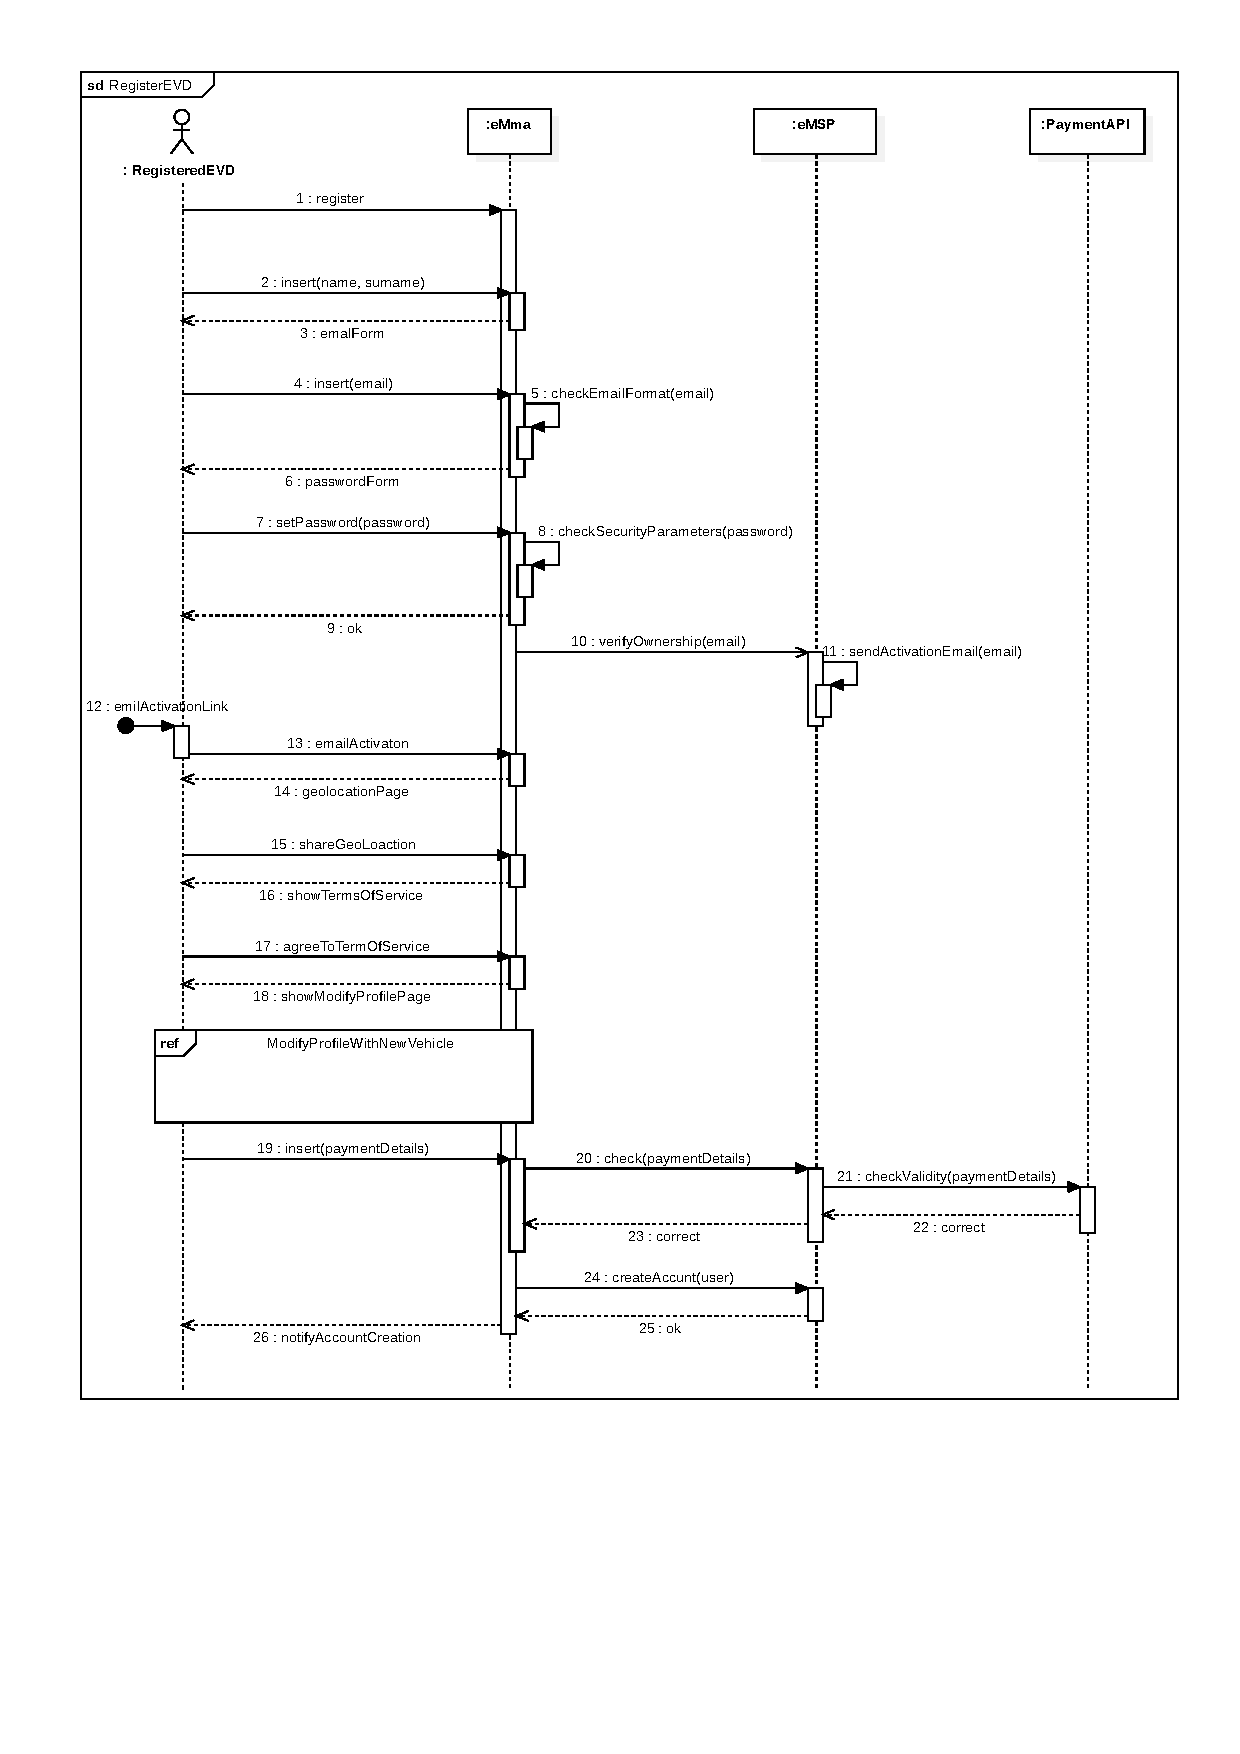
\includegraphics[width=1\textwidth, trim={1cm 5cm 0 1.2cm}, clip]{Images/cp3/seqDiagrams/RegisterEVD.pdf}
    \caption{RegisterEVD sequence diagram}
\end{figure}
\pagebreak

\paragraph{Log in the system}
\begin{center}
    \begin{longtable}{p{4cm} p{11cm}}
    \multicolumn{2}{r}{\itshape{continue on the next page}}\\
    \endfoot 
    \\
    \endlastfoot
    \hline
     Use case name &  LogIn\\
     \hline
     Actor & Registered user (EVD or CPO)\\
     \hline
     Entry condition &  The user is not logged in the system and wants to log in\\
     \hline
     Event flow &   1. The user accesses the eMma \newline
                    2. The eMma shows the log in page \newline
                    3. The user inserts the log in details \newline
                    4. The system checks the correctness of the log in details \newline
                    5. The eMma logs in the user and shows the homepage\\
     \hline
     Exit condition & The user is logged in and is shown the homepage of the eMma \\
     \hline
     Exceptions &  If the credentials are not correct the user receives an error message and the login operation is not successful \\
     \hline
     Special requirements &  After inserting the credentials, the login details must be checked and the eMall homepage must be shown in less than 2 seconds \\
     \hline
    \caption{LogIn}
    \label{tab:LogIn}
    \end{longtable}
\end{center}

\begin{figure}[H]
    \centering
    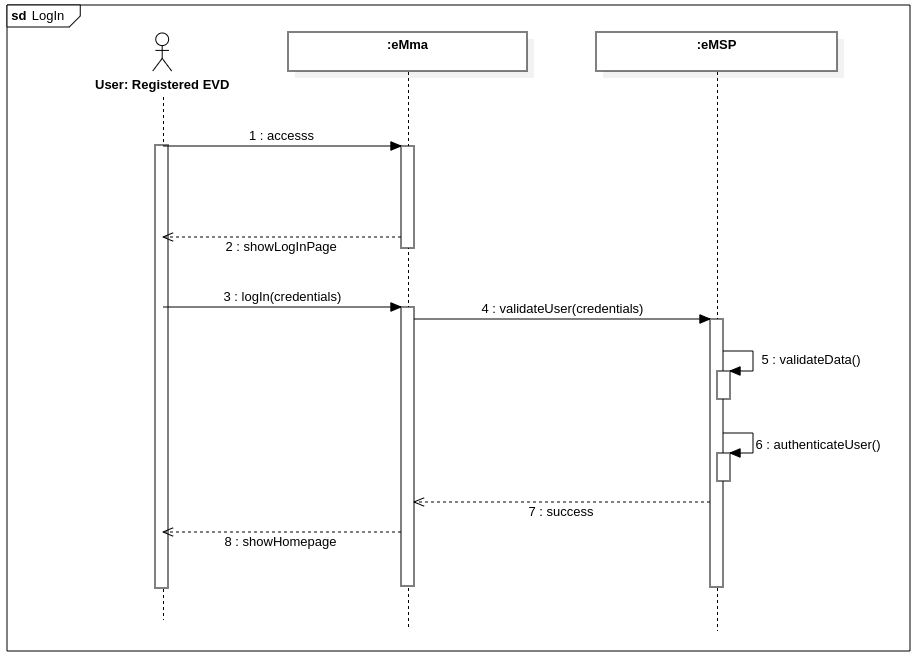
\includegraphics[width=0.8\textwidth]{Images/cp3/LogInSD.png}
    \caption{LogIn sequence diagram}
\end{figure}

\paragraph{Booking a charging point}
\begin{center}
    \begin{longtable}{p{4cm} p{11cm}}
    \multicolumn{2}{r}{\itshape{continue on the next page}}\\
    \endfoot 
    \\
    \endlastfoot
    \hline
     Use case name &  BookChargingPoint\\
     \hline
     Actor & EVD \\
     \hline
     Entry condition &   The EVD is logged in the eMma and on the homepage\\
     \hline
     Event flow &
        1. The EVD performs <<include>>VisualizeStations \newline
        2. The EVD selects to book a charging session from a charging station \newline
        3. eMma shows a list of available charging points with the following information:
            \begin{adjustwidth}{0.5cm}{}
                \begin{itemize}
                    \item The type of charging (AC/DC)
                    \item The type of the socket (type 1, type 2, CCS, CHAdeMO, etc.)
                    \item The charging speed denoted in kW and km/h (km gained per one hour of charge)
                    \item The price for kWh
                    \item The price for unlocking the socket
                \end{itemize}
            \end{adjustwidth}
        4. EVD selects the charging point that suits his needs \newline
        5. The EVD set the date, the starting and ending time of the charging session \newline
        6. eMma shows to the EVD a summary of the booking and asks the EVD for confirmation \newline
        7. EVD confirms the booking \newline
        8. The system processes the booking request \newline
        9. eMma notifies the EVD about the success of the booking operation\\
     \hline
     Exit condition &  Booking is registered\\
     \hline
     Exceptions &
        If the booking confirmation fails, eMma shall notify the user about the occurrence of an error and should bring the view back to the list of available charging points\\
     \hline
     Special requirements &  
        The system processes the booking request and sends a notification message in less than 5 seconds. Also, at each interaction the response of the eMma is perceived as immediate, taking less than 2 seconds to perform any operation\\
     \hline
    \caption{BookingChargingPoint}
    \label{tab:BookingChargingPoint}
    \end{longtable}
\end{center}
\begin{figure}[H]
    \centering
    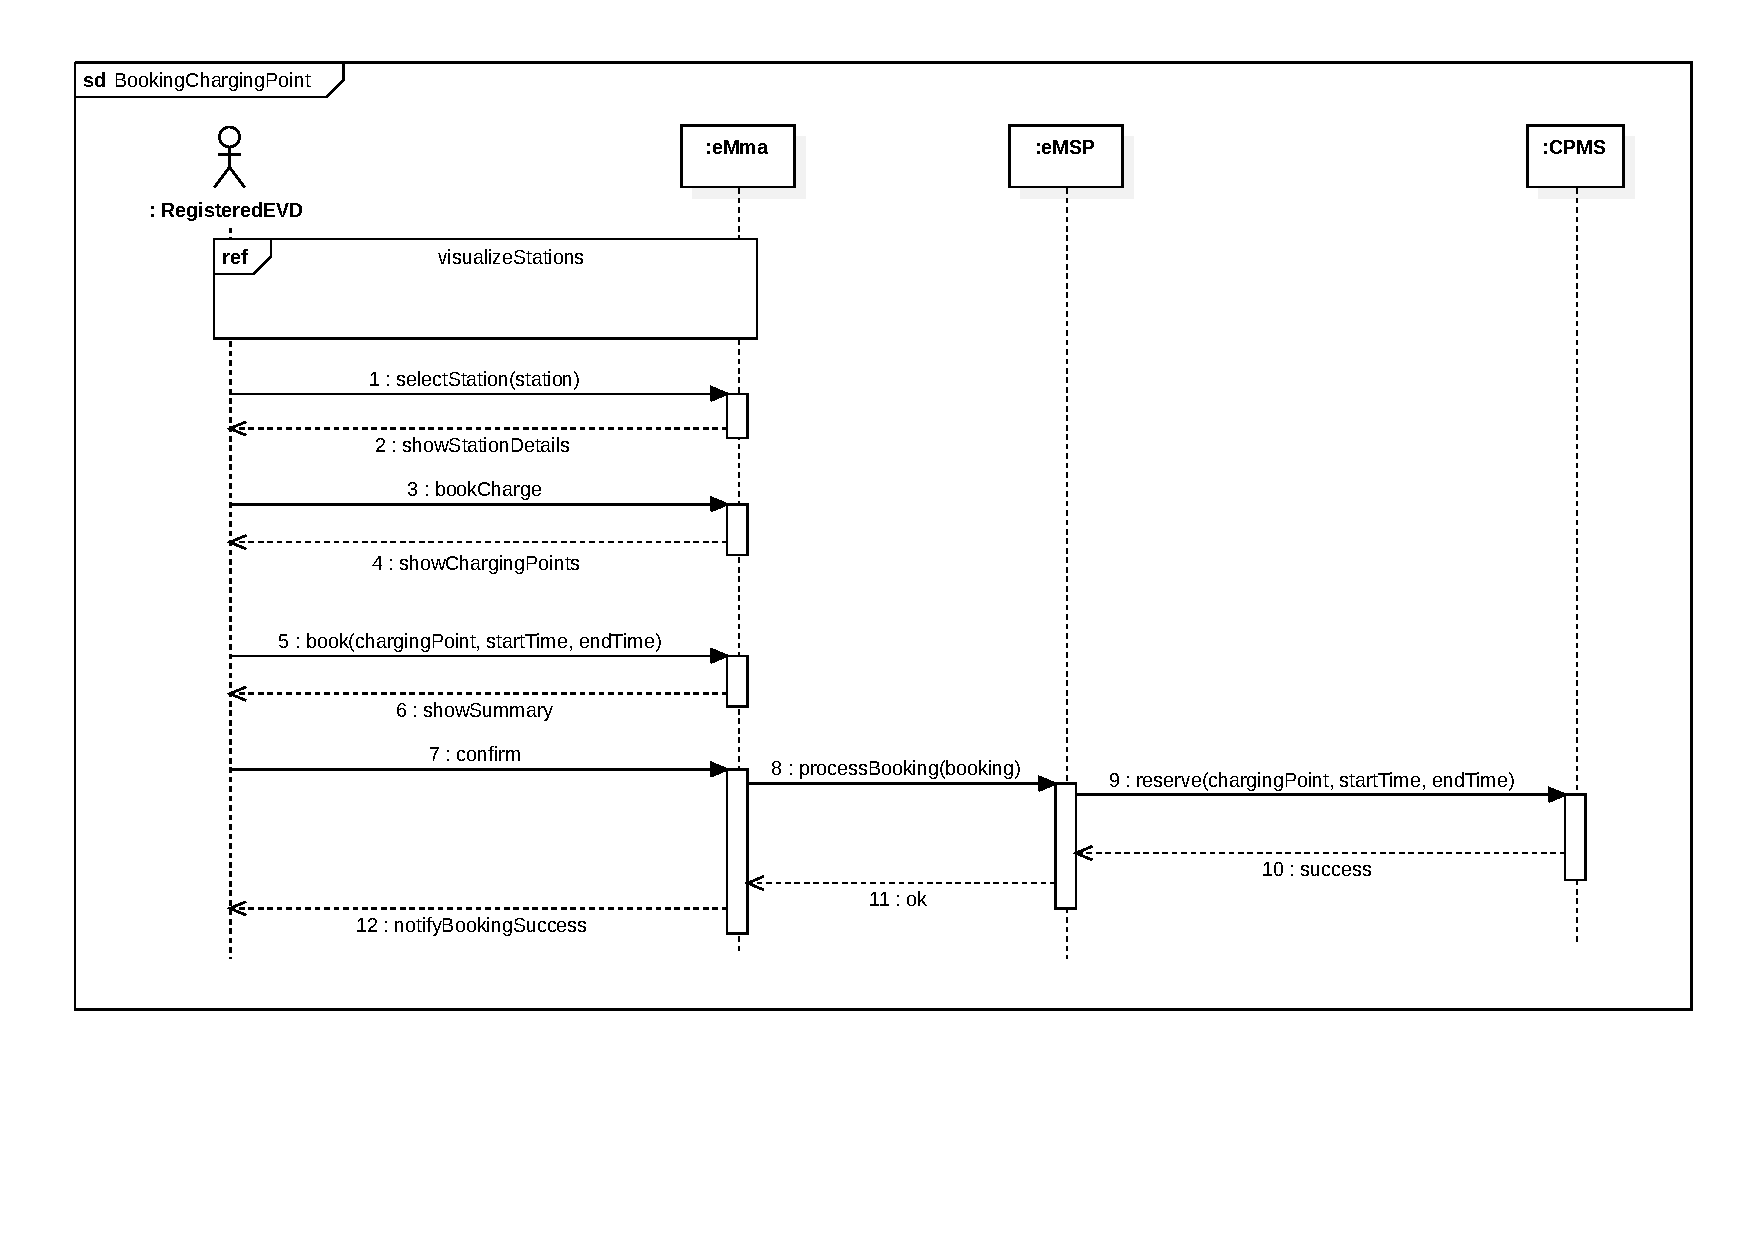
\includegraphics[width=\textwidth, trim={0 3cm 0 0}, clip]{Images/cp3/seqDiagrams/BookChargingPoint.pdf}
    \caption{BookingChargingPoint sequence diagram}
\end{figure}

\paragraph{Cancel a booking}
\begin{center}
    \begin{longtable}{p{4cm} p{11cm}}
    \multicolumn{2}{r}{\itshape{continue on the next page}}\\
    \endfoot 
    \\
    \endlastfoot
    \hline
     Use case name &  CancelBooking\\
     \hline
     Actor & EVD \\
     \hline
     Entry condition &   The EVD is logged in the eMma and on the homepage\\
     \hline
     Event flow &
        1. EVD selects upcoming charging section \newline
        2. eMma shows an entry with details about the upcoming charging booking \newline
        3. EVD selects the entry \newline
        4. eMma allows the EVD the possibility to cancel the booking \newline
        5. EVD selects to cancel the booking \newline
        6. eMma asks for confirmation \newline
        7. EVD confirms \newline
        8. eMma notifies the EVD about the canceling and sends information to the eMSP about the canceling\\
     \hline
     Exit condition &  The booking is cancelled\\
     \hline
     Exceptions &
        If the booking confirmation fails, eMma shall notify the user about the occurrence of an error and should bring the view back to the list of available charging points
     \\
     \hline
     Special requirements & 
        The EVD is notified about the booking cancellation in less than 2 seconds, for the operation to be perceived as immediate\\
     \hline
    \caption{CancelBooking}
    \label{tab:CancelBooking}
    \end{longtable}
\end{center}

\begin{figure}[H]
    \centering
    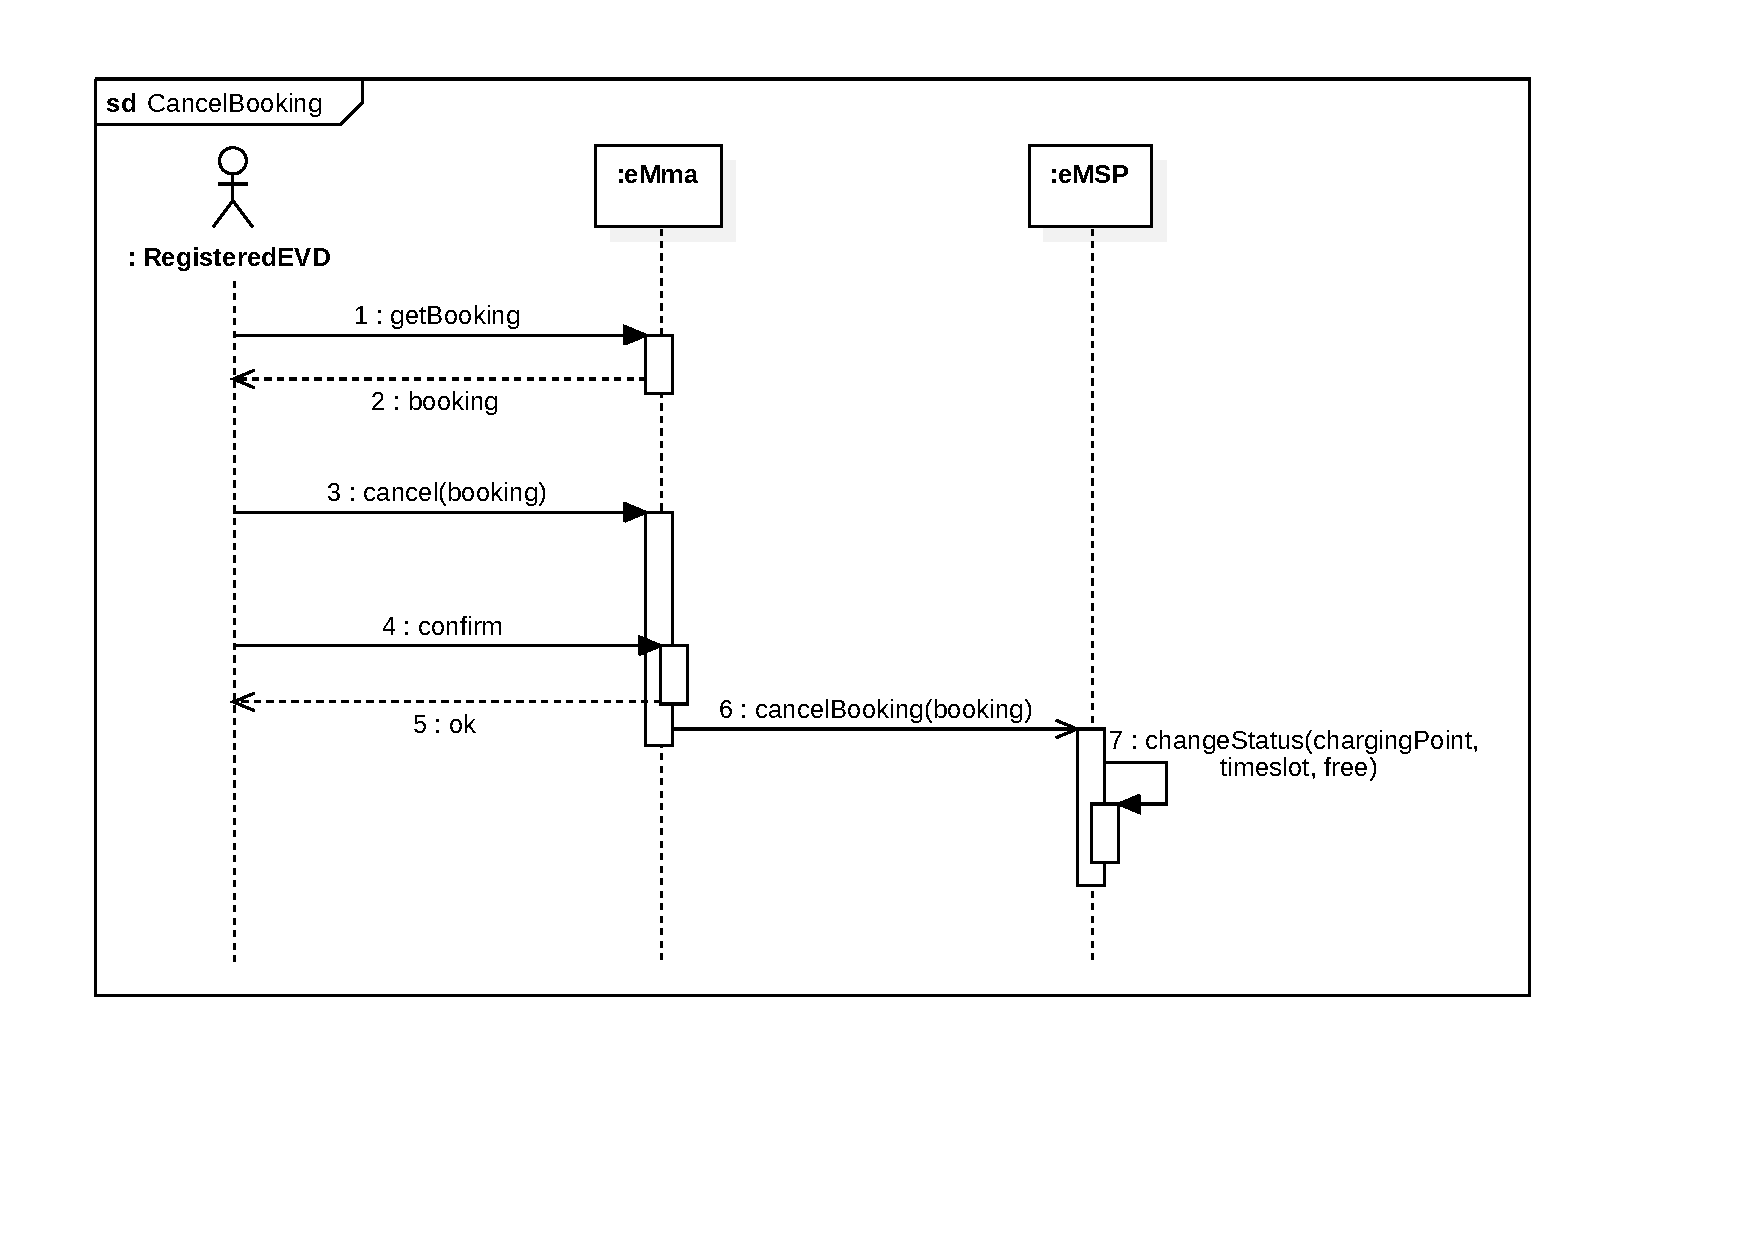
\includegraphics[width= 1\textwidth, trim={1.5cm 3.5cm 3cm 1cm}, clip]{Images/cp3/seqDiagrams/CancelBooking.pdf}
    \caption{CancelBooking sequence diagram}
\end{figure}

\clearpage
\paragraph{Visualize charging history}
\begin{center}
    \begin{longtable}{p{4cm} p{11cm}}
    \multicolumn{2}{r}{\itshape{continue on the next page}}\\
    \endfoot 
    \\
    \endlastfoot
    \hline
     Use case name &  VisualizeChargingHistory\\
     \hline
     Actor & Registered EVD \\
     \hline
     Entry condition & User is logged in eMma  \\
     \hline
     Event flow & 
        1. EVD selects to view the charging history section \newline
        2. eMma shows a view containing details about the upcoming charge booking with it's details and a list \newline
        3. EVD confirms to see the charging history \newline
        4. eMma shows a chronologically ordered list of all the previous charging sessions processed throught the system. Each element on the list contains details about:
            \begin{adjustwidth}{0.5cm}{}
                \begin{itemize}
                    \item the EV involved %If there are more vehicles
                    \item the date and time
                    \item the location
                    \item how long the charging lasted
                    \item how many KWh were charged
                    \item type of socket used
                    \item cost per kWh of the charge
                    \item total cost of the charge
                \end{itemize}
            \end{adjustwidth}
        5. EVD can select the filter option, to have a different visualization, based on what he is curious about, for example grouping the visualization on the EV involved in the charge \newline
        6. eMall shows the list of the previous charging sessions, with the details, according to the selected filter\\
     \hline
     Exit condition & The EVD exits from the visualization history and the eMall reloads the homepage \\
     \hline
     Exceptions & 
        a. If the user hasn't got any imminent charges booked, the eMma shows directly the charging history \newline
        b. If the user hasn't done any charges yet with the system, then the eMma shows an empty page \\
     \hline
     Special requirements &  The eMma shows the history in less than 5 seconds, for every chosen filtering option\\
     \hline
    \caption{VisualizeChargingHistory}
    \label{tab:VisualizeChargingHistory}
    \end{longtable}
\end{center}

\begin{figure}[H]
    \centering
    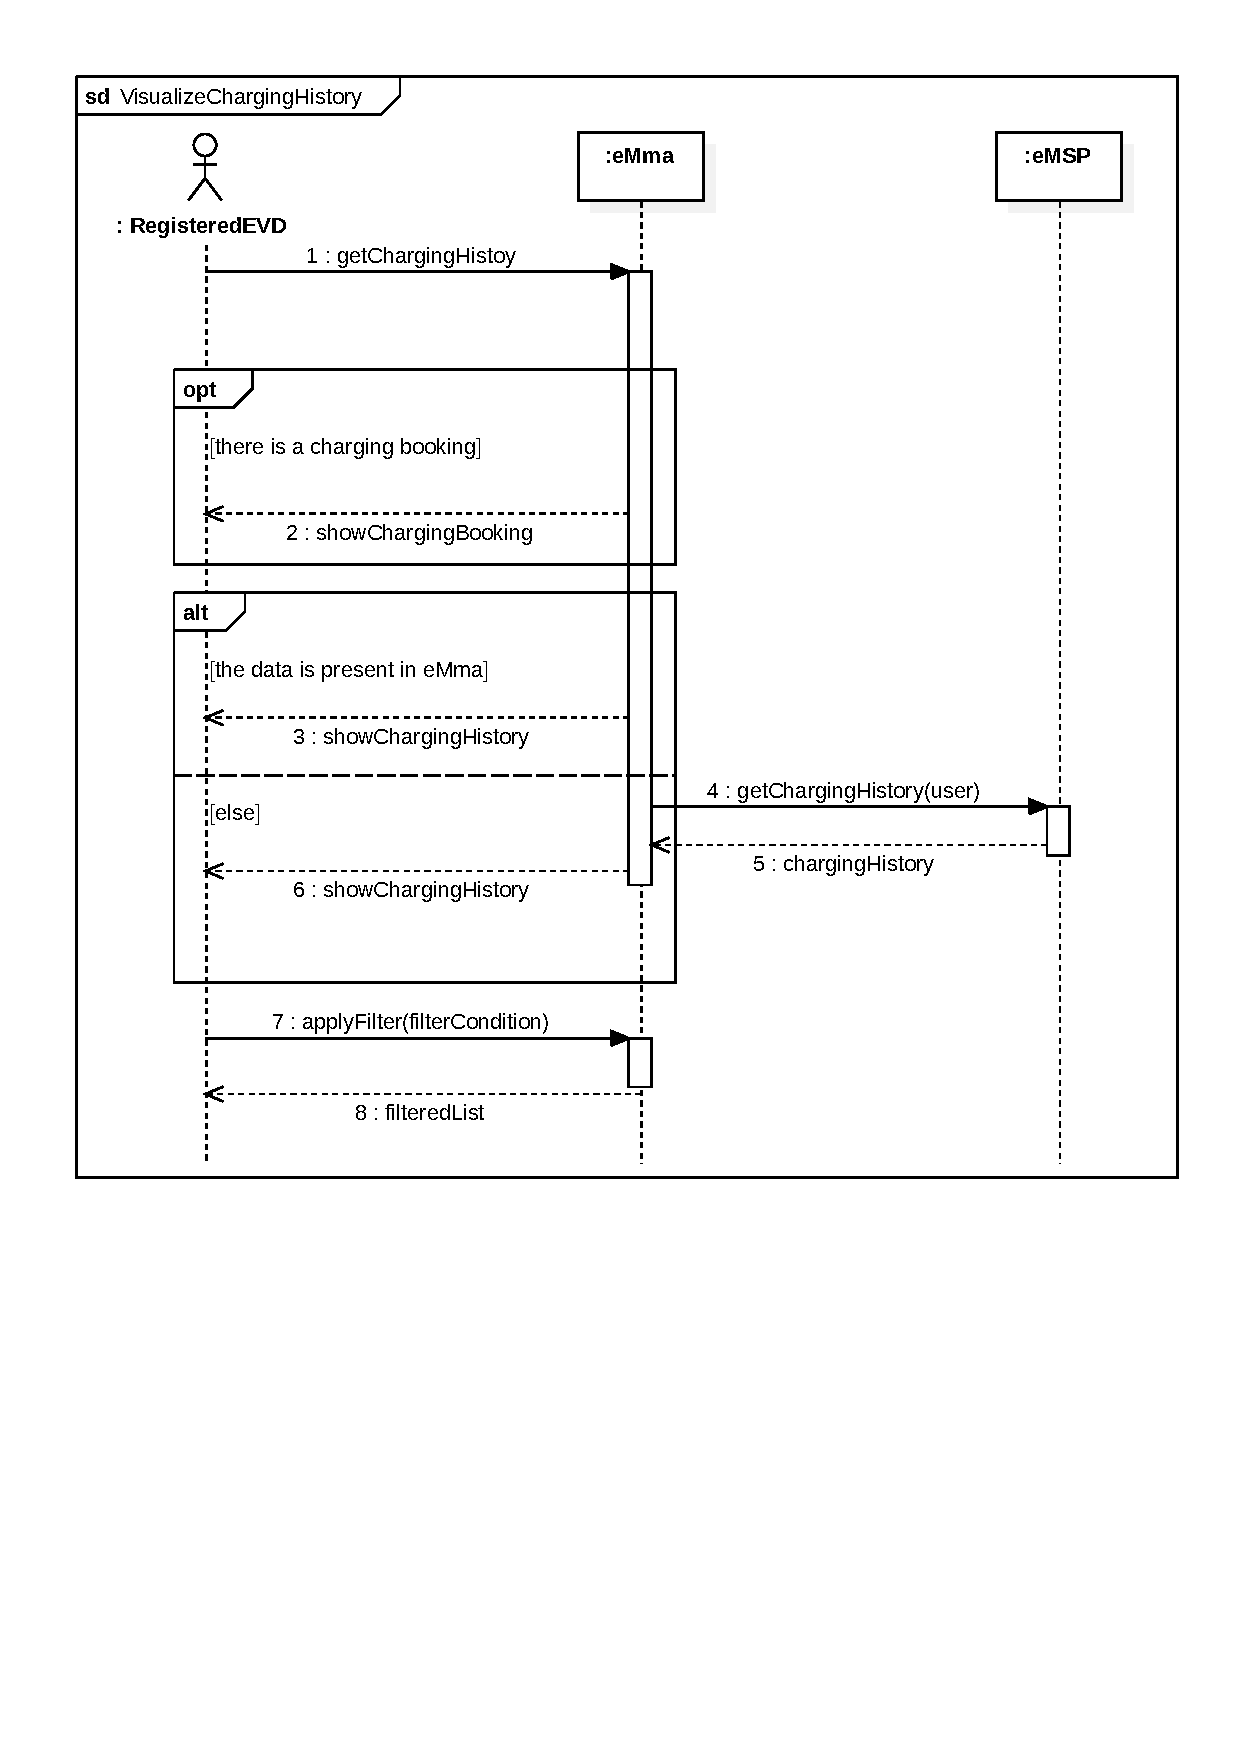
\includegraphics[width=\textwidth, trim={0 9cm 0 0}, clip]{Images/cp3/seqDiagrams/VisualizeChargingHistory.pdf}
    \caption{VisualizeChargingHistory sequence diagram}
\end{figure}

\clearpage
\paragraph{Start a charging session}
\begin{center}
    \begin{longtable}{p{4cm} p{11cm}}
    \multicolumn{2}{r}{\itshape{continue on the next page}}\\
    \endfoot 
    \\
    \endlastfoot
    \hline
     Use case name &  ChargeNow\\
     \hline
     Actor & EVD \\
     \hline
     Entry condition & The EVD is on the homepage of the eMma and the status of the charging point is free \\
     \hline
     Event flow &   
        1. The EVD selects the section used for the immediate charging operation \newline
        2. The EVD inserts the eMci code in the eMma and confirms the operation \newline
        3. The eMall checks the correctness of the code and unlocks the charging point \newline
        4. The system changes the status of the charging point from free to occupied \newline   
        5. The eMma sends a success notification message to the user, to inform him that the charging point is ready and is waiting for the connector to be plugged in\\
     \hline
     Exit condition &  The EVD plugs in the connector and the system actually starts the charging process \\
     \hline
     Exceptions &   
        a. If the EVD doesn't insert the correct code, the eMall doesn't unlock the charging point and the eMma returns a warning message, allowing the user to reinsert the code\newline
        b. If the user doesn't insert the plug in less than 5 minutes, the operation is deleted, and the charging point status return to free \newline
        c. If the EVD is not registered, when confirming the code, he has to make a deposit in order to use the charger\\ 
     \hline
     Special requirements & After inserting the code, the eMall does all the necessary checks and changes the status of the charging point in less than 2 seconds, so the service can be perceived as fast and responsive. Also, the system has to start the charging of the EVD in less than 2 seconds, for the same reason \\
     \hline
    \caption{ChargeNow}
    \label{tab:ChargeNow}
    \end{longtable}
\end{center}

\begin{figure}[H]
    \centering
    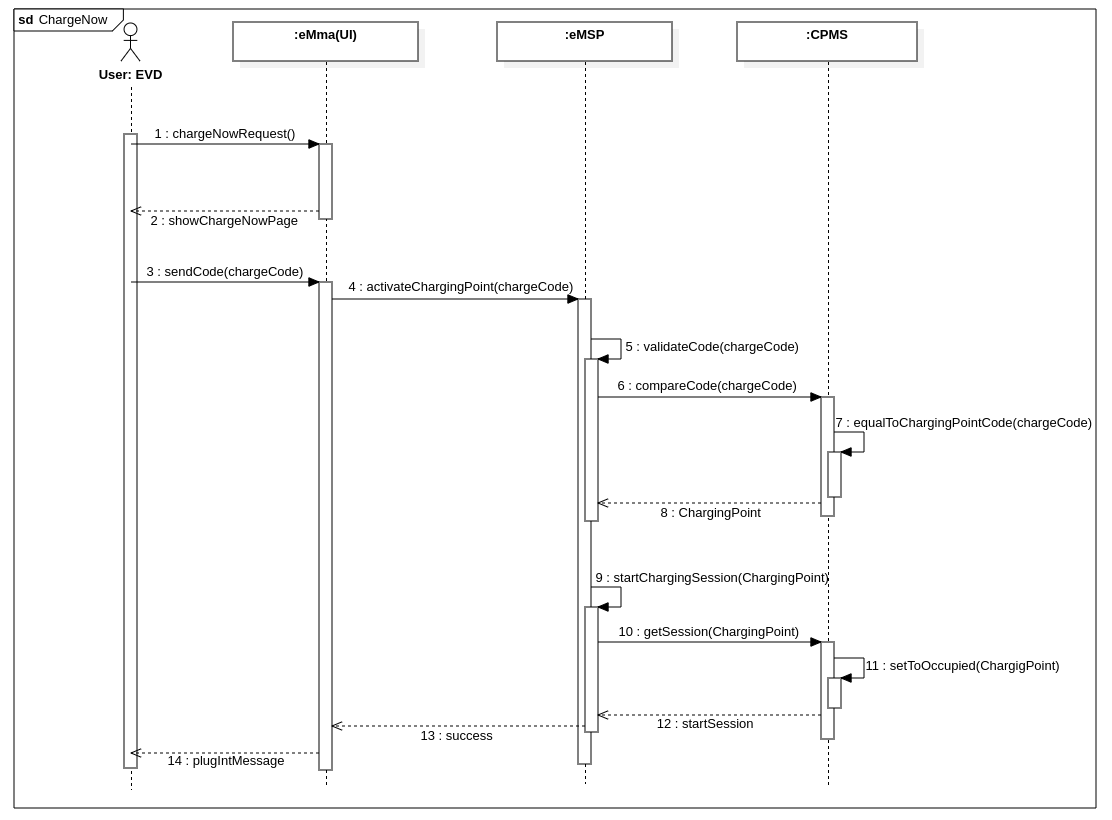
\includegraphics[width=1\textwidth]{Images/cp3/ChargeNowSD.png}
    \caption{ChargeNow sequence diagram}
\end{figure}

\clearpage
\paragraph{Update profile details adding a new vehicle}
\begin{center}
    \begin{longtable}{p{4cm} p{11cm}}
    \multicolumn{2}{r}{\itshape{continue on the next page}}\\
    \endfoot 
    \\
    \endlastfoot
    \hline
     Use case name &  ModifyProfileWithNewVehicle\\
     \hline
     Actor & Registered EVD \\
     \hline
     Entry condition & The EVD is logged in the eMma and on the homepage \\
     \hline
     Event flow &   1. The EVD enters on his profile page \newline
                    2. The system shows the profile page with personal information and EV's details \newline
                    3. The EVD selects the update option \newline
                    4. The eMma shows a page with different buttons from which to choose the update action \newline
                    5. The EVD chooses as update action, the one that represents the insertion of a new vehicle \newline
                    6. The mobile app shows a form with different fields to fill up\newline
                    7. The EVD inserts the data about the new EV: inserts the type of EV, the supported inlet type of the EV and the presence of the rectifier, the capacity of the battery, the supported power levels and the supported current levels \newline
                    8. The EVD confirms the operation, submitting the form \newline
                    9. The eMall saves the data and associates them to the EVD's profile \newline
                    10. The system reloads the profile page with the new vehicle information \\
     \hline
     Exit condition &  The new EV is associated to the user information already saved in the system, and the eMma reloads the profile page with the new EV's details\\
     \hline
     Exceptions &   
        a. If the EVD doesn't insert all the mandatory information, after clicking the 'Ok' button the system gives an explicit error message with the missing data, and the user can continue to complete the form \newline
        b. If at any time the user wants to exit the form, the application allows it, but all the data inserted so far are lost \\
     \hline
     Special requirements & After the EVD's confirmation, the system has to save the data and reload the profile page in less than 10 seconds \\
     \hline
    \caption{ModifyProfileWithNewVehicle}
    \label{tab:ModifyProfileWithNewVehicle}
    \end{longtable}
\end{center}

\paragraph{Update profile details deleting vehicle}
\begin{center}
    \begin{longtable}{p{4cm} p{11cm}}
    \multicolumn{2}{r}{\itshape{continue on the next page}}\\
    \endfoot 
    \\
    \endlastfoot
    \hline
     Use case name &  ModifyProfileDeletingVehicle\\
     \hline
     Actor & Registered EVD \\
     \hline
     Entry condition & The EVD is logged in the eMma and on the homepage \\
     \hline
     Event flow &   1. The EVD enters on his profile page \newline
                    2. The system shows the profile page with personal information and EV's details \newline
                    3. The EVD selects the update option \newline 
                    4. The eMma shows a page with different buttons from which to choose the update action \newline
                    5. The EVD selects the action that represents the operation of deleting  a vehicle \newline
                    6. The mobile app shows a form with the list of the registered vehicles \newline
                    7. The EVD selects the EV he wants to delete \newline
                    8. The EVD confirms the operation submitting his choice \newline
                    9. The eMall retrieves the data of the user and deletes the selected vehicle \newline
                    10. The system reloads the profile page, in which the deleted vehicle is no more present \\
     \hline
     Exit condition &  The EV is deleted from the data associated to the EVD and the profile page is reloaded \\
     \hline
     Exceptions &  
        a. If the EVD doesn't select an EV to delete from the list, after clicking the 'Ok' button the system gives an error message, and the user has to select a vehicle or cancel the operation\newline
        b. If the user wants to exit without selecting an EV, the application allows it, and no vehicle will be deleted from the profile\\
     \hline
     Special requirements &  After the EVD's confirmation, the system has to delete the vehicle from the EVD's data and reload the profile page in less than 3 seconds \\
     \hline
    \caption{ModifyProfileDeletingVehicle}
    \label{tab:ModifyProfileDeletingVehicle}
    \end{longtable}
\end{center}

\paragraph{Update profile modifying personal data}
\begin{center}
    \begin{longtable}{p{4cm} p{11cm}}
    \multicolumn{2}{r}{\itshape{continue on the next page}}\\
    \endfoot 
    \\
    \endlastfoot
    \hline
     Use case name &  ModifyProfilePersonalData\\
     \hline
     Actor & Registered EVD \\
     \hline
     Entry condition & The EVD is logged in the eMma and on the homepage \\
     \hline
     Event flow &   1. The EVD enters on his profile page \newline
                    2. The system shows the profile page with personal information and EV's details \newline
                    3. The EVD selects the update option \newline
                    4. The eMma shows a page with different buttons from which to choose the update action \newline
                    5. The EVD selects the option the represent the operation of updating the profile personal data \newline
                    6. The mobile app shows a form, already filled up with the personal data \newline
                    7. The EVD can modify the elements of the form, for example the email, the name, the payment details \newline
                    8. The EVD, after modifying some data, confirms the operation and submits the form \newline
                    9. The eMall checks (internally and externally using APIs) and updates the data that have been changed, saving the correct information associated to the EVD's profile \newline
                    10. The system reloads the profile page with the new data \\
     \hline
     Exit condition & The system saves the new data, discarding the old ones, and the eMma reloads the profile page with the updated details\\
     \hline
     Exceptions &   
        a. If the EVD doesn't change any data of the form, after clicking the 'Ok' button the system reloads the profile page showing all the data present before the operation \newline
        b. If at any time the user wants to exit the form, the application allows it, but all the data inserted so far are lost, keeping the last personal details \newline
        c. If the EVD doesn't confirm the operation from the eMma or from the external applications, the updating request is deleted after 10 minutes, and the operation has to be restarted \\
     \hline
     Special requirements & After clicking the 'Confirm' button the system has to save the updated data and reload the profile page in less than 10 seconds \\
     \hline
    \caption{ModifyProfilePersonalData}
    \label{tab:ModifyProfilePersonalData}
    \end{longtable}
\end{center}
We show only a sequence diagram for all the use cases regarding the modification of the profile, because even if the data which are modified are different and some actions and checks can change, overall the event flow is the same in all of them. So, the following diagram treats only the action in a general way, representing with it all the possible operations.
\begin{figure}[H]
    \centering
    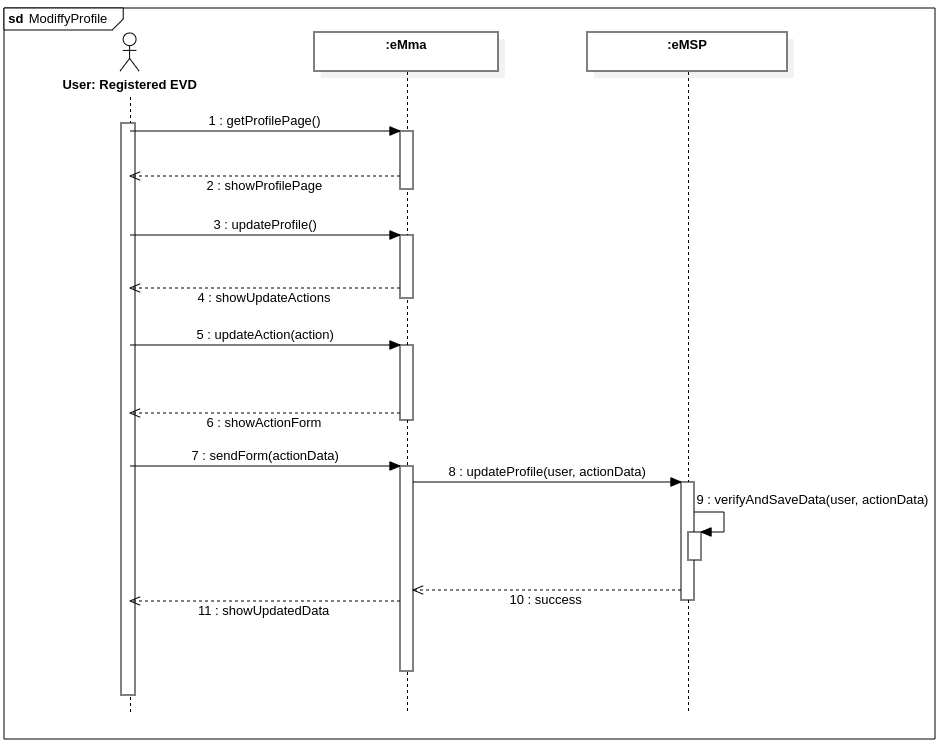
\includegraphics[width=1\textwidth]{Images/cp3/ModifyProfileSD.png}
    \caption{ModifyProfile sequence diagram: the use cases ModifyProfileNewVehicle, ModifyProfileDeleteVehicle and ModifyProfilePersonalData are grouped in this diagram}
\end{figure}

\paragraph{Visualize charging stations on the map}
\begin{center}
    \begin{longtable}{p{4cm} p{11cm}}
    \multicolumn{2}{r}{\itshape{continue on the next page}}\\
    \endfoot 
    \\
    \endlastfoot
    \hline
     Use case name &  VisualizeStations\\
     \hline
     Actor & Registered EVD or unregistered EVD \\
     \hline
     Entry condition & The EVD is on the eMma homepage \\
     \hline
     Event flow &   1. On the homepage the eMma shows the map of the territory, based on the location shared                by the mobile phone of the EVD \newline
                    2. The map shows the charging stations nearby the position of the EVD \newline
                    3. The EVD clicks on one of the charging stations presented on the map \newline
                    4. The eMma shows a page with the information related to the selected charging station:
                    \begin{adjustwidth}{0.5cm}{}
                        \begin{itemize}
                                \item The name of the charging station
                                \item the rating of the charging station
                                \item indication about the available sockets types and their number
                                \item contact details
                                \item address of the charging station
                                \item any directions on how to handle the charging process
                                \item Reviews about the charging station
                                \item the presence of any special offer
                        \end{itemize}
                    \end{adjustwidth}   
                    5. The EVD can, also, insert other locations in which to visualize the stations on the map
     \\
     \hline
     Exit condition & The EVD exits the homepage or closes the application \\
     \hline
     Exceptions &   a. If the EVD clicks on the map on an area without charging stations, no charging station will appear on the map \newline
                    b. If at any time the user wants to exit the eMma, the application allows it, and at the following access the action restarts from the homepage \\
     \hline
     Special requirements & After the EVD clicks on the map, the charging stations are shown in less than 2 seconds. As well, when the EVD clicks on the charging stations the related data are shown in less than 2 seconds, so the application can be perceived as fast \\
     \hline
    \caption{VisualizeStations}
    \label{tab:VisualizeStations}
    \end{longtable}
\end{center}
\begin{figure}[H]
    \centering
    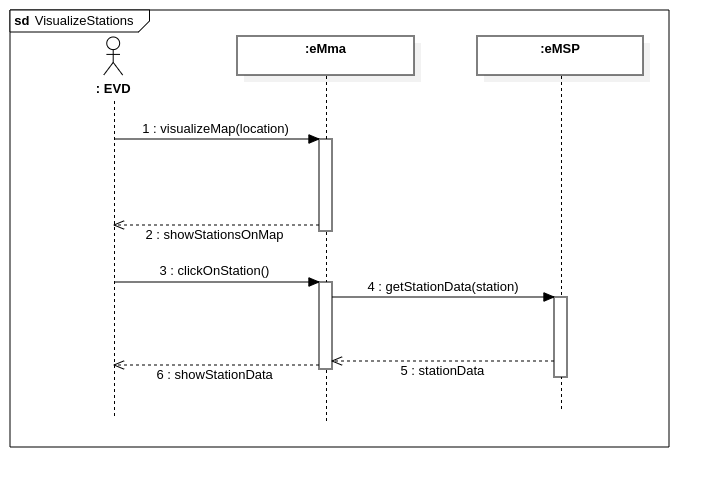
\includegraphics[width=1\textwidth]{Images/cp3/seqDiagrams/VisualizeStations.png}
    \caption{VisualizeStations sequence diagram}
\end{figure}

\clearpage
\paragraph{Terminate charging process}
\begin{center}
    \begin{longtable}{p{4cm} p{11cm}}
    \multicolumn{2}{r}{\itshape{continue on the next page}}\\
    \endfoot 
    \\
    \endlastfoot
    \hline
     Use case name &  TerminateCharging\\
     \hline
     Actor & eMma \\
     \hline
     Entry condition & Charging is almost completed (over 80\%) \\
     \hline
     Event flow &   1. The eMma sends a notification that the charging is almost completed \newline
                    2. The EVD opens the notification \newline
                    3. The EVD confirms the termination \newline
                    4. The eMall stops the charging session \newline
                    5. The eMall initiates the payment operation \newline
                    6. The EVD selects from the eMma the payment method and confirms the operation \newline
                    7. The eMall communicates with external APIs in order to complete the payment \newline
                    8. The eMall sends a message notifying the successful payment \newline
                    9. The EVD confirms the termination of the operation \newline
                    10. The eMma asks for a review of the service \newline
                    11. The EVD can leave a review and a comment \newline
                    12. The EVD unplugs the EV from the charging point
     \\
     \hline
     Exit condition & The EVD unplugs the EV after paying for the charging session\\
     \hline
     Exceptions &   
        a. If the EVD doesn't unplug the EV in less than 10 minutes, once the EV is fully charged, at the original price is added an additional cost for each minute in which the charging point is occupied \newline
        b. If the EVD wants to stop the charge at any moment, even if the battery is not completely charged he can do so, paying for the obtained service \newline
        c. If the payment is not successful the eMma sends a warning and requests again the payment method
        \\
     \hline
     Special requirements & After every confirmation the system responds in less than 2 seconds. The eMall also needs less than 20 seconds to complete the payment, communicating with external APIs \\
     \hline
    \caption{TerminateCharging}
    \label{tab:TerminateCharging}
    \end{longtable}
\end{center}
\begin{figure}[H]
    \centering
    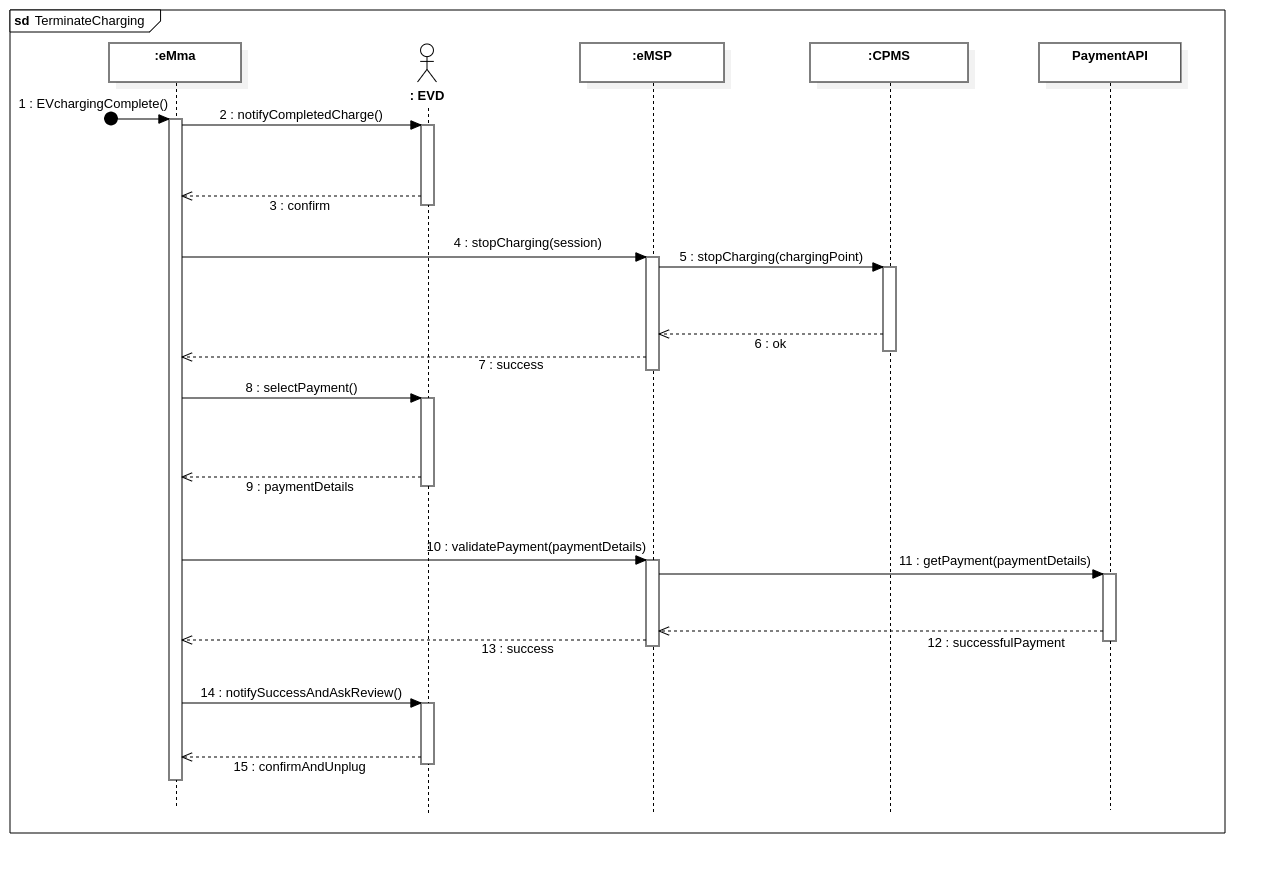
\includegraphics[width=1\textwidth]{Images/cp3/seqDiagrams/TerminateCharging.png}
    \caption{TerminateCharging sequence diagram}
\end{figure}

\subsection{CPO's use cases}
\begin{figure}[H]
    \centering
    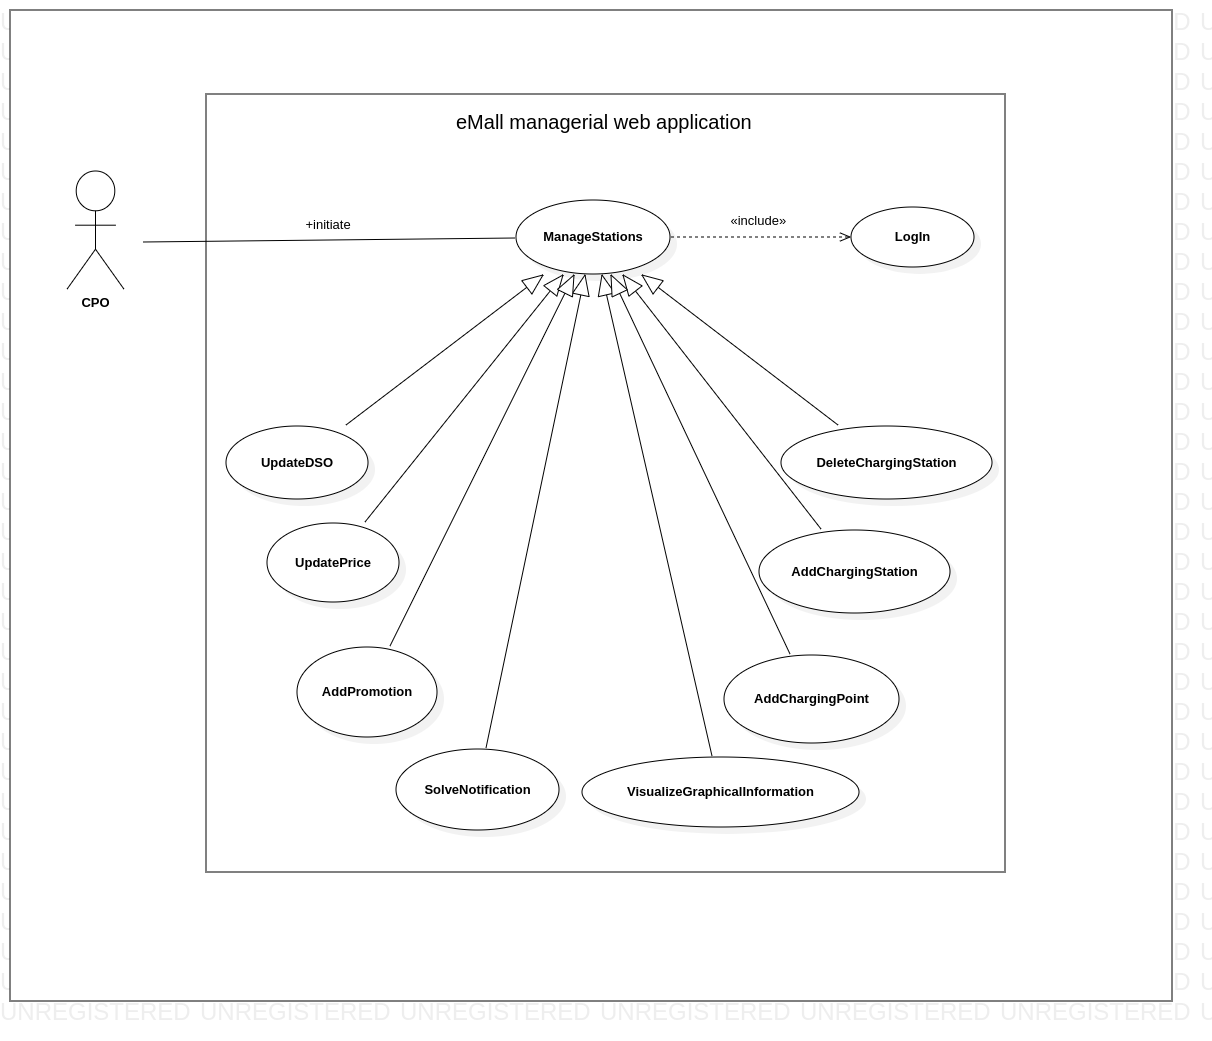
\includegraphics[width= 0.9\textwidth, trim={1cm 2cm 2cm 1cm}, clip]{Images/cp3/UseCaseDiagramCPO.png}
    \caption{Use cases diagram of the CPO}
\end{figure}
We can notice that the CPO actor activities are concentrated on the managing of the charging stations. All the operations specify the general one 'ManageStations', and there can be many others beyond the ones that are presented here, because the CPO can update and add a lot of data, which are then sent to the CPMS. We decided to concentrate our analyses on the main features that regard the system, such as updates regarding the DSO from which to acquire energy, updates of the prices and the special offers, and other essential operations regarding the stations and the related charging points and batteries.

\clearpage
\paragraph{Manage the charging stations}
\begin{center}
    \begin{longtable}{p{4cm} p{11cm}}
    \multicolumn{2}{r}{\itshape{continue on the next page}}\\
    \endfoot 
    \\
    \endlastfoot
    \hline
     Use case name &  ManageStations\\
     \hline
     Actor & CPO \\
     \hline
     Entry condition & The CPO is logged in the web application of the eMall and on the homepage \\
     \hline
     Event flow &   
        1. On the homepage the eMall shows to the CPO the charging stations associated to the company registration and any notification on the stations \newline
        2. The CPO clicks on a charging station or on a notification \newline 
        3. The system shows a form with the details of the charging station and if there are notifications regarding the station the interested parts of the form are highlighted in red \newline
        4. The CPO can click on any part of the form and modify the data of the station \newline
        5. The CPO confirms the operation \newline
        6. The system checks and saves the new data related to the charging station \newline
        7. The system sends a notification message informing of the success of the operation \newline
        8. The system loads a page showing the charging station with the new associated information\\
     \hline
     Exit condition &  The CPO closes the page loaded by the system with the updated data of the charging station, returning to the homepage \\
     \hline
     Exceptions &   
        a. If the CPO doesn't modify anything on the form before submitting it, the eMall sends a message which informs that the data have not been modified, and returns to the homepage \newline
         b. If at any time the CPO wants to exit, the application allows it, and no changes will be applied if the procedure wasn't completed \\
     \hline
     Special requirements & After the CPO confirms the operation, the charging station with the related details is updated and shown on a new page in less than 2 seconds, in order for the application to be perceived as fast and responsive \\
     \hline
    \caption{ManageStations}
    \label{tab:ManageStations}
    \end{longtable}
\end{center}

\begin{figure}[H]
    \centering
    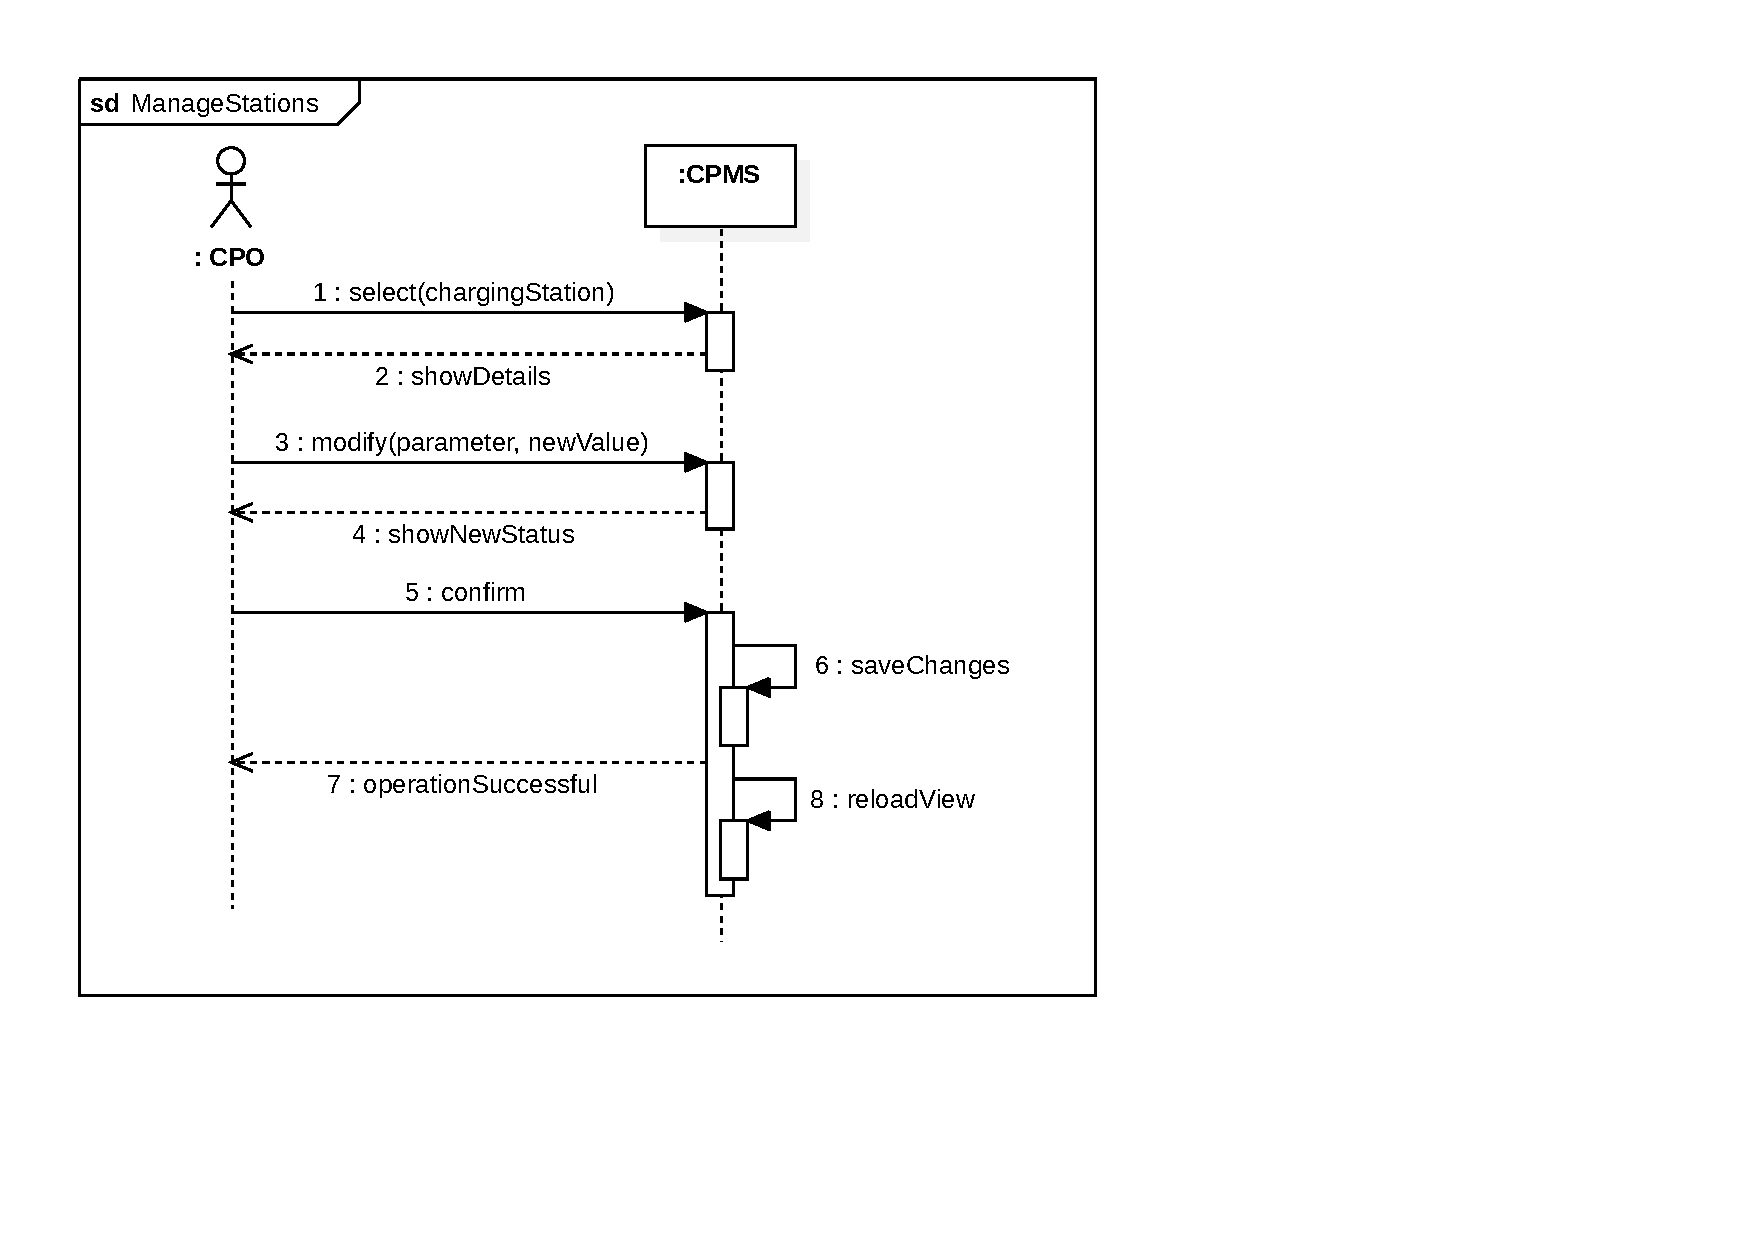
\includegraphics[width=0.8\textwidth, trim={0 4cm 11cm 0}, clip]{Images/cp3/seqDiagrams/ManageStations.pdf}
    \caption{ManageStations sequence diagram}
\end{figure}

The use case about the CPO managing the charging stations, is a generic use case, that can be further analyzed considering the actions that the CPO actually performs on the system, to manage the stations. In the following use cases, we specialize some of these interactions, as already mentioned at the beginning of this section, showing available functionalities of the web application of the eMall. 
%TODO: @Fabio sequence diagrams of the other CPO use cases or leave this line
The sequence diagrams of the next use cases exhibit a similar event-flow as the one reported for the general interaction of the CPO with the system, so they will not be added to this document.

\clearpage
\paragraph{Update the DSO of a charging station}
\begin{center}
    \begin{longtable}{p{4cm} p{11cm}}
    \multicolumn{2}{r}{\itshape{continue on the next page}}\\
    \endfoot 
    \\
    \endlastfoot
    \hline
     Use case name &  UpdateDSO\\
     \hline
     Actor & CPO \\
     \hline
     Entry condition & The CPO is logged in the web application of the eMall and on the homepage \\
     \hline
     Event flow &   1. On the homepage the eMall shows to the CPO the charging stations associated to the company                   registration and any notification on the stations \newline
                    2. The CPO clicks on a charging station \newline 
                    3. The system shows a form with the details of the station \newline
                    4. The CPO clicks on the 'DSO' cell present in the form \newline
                    5. The system shows a new sub-page with the available DSOs and the respective information: for each DSO the page shows the energy resources, their capacity and their prices \newline
                    6. The CPO selects the DSO and the energy source he wants to use for the charging station \newline
                    7. The CPO confirms the operation \newline
                    8. The web application returns to the form of the charging station with the new selected DSO information \newline
                    9. The CPO confirms the operation \newline
                    10. The system checks and saves the new data related to the charging station \newline
                    11. The system sends a notification message informing of the success of the operation \newline
                    12. The system loads a page showing the charging station with the new associated information\\
     \hline
     Exit condition &  The CPO closes the page loaded by the system with the updated data of the charging station, returning to the homepage \\
     \hline
     Exceptions &   a. If the CPO doesn't modify anything on the form before submitting it, the eMall sends a                       message which informs that the data have not been modified, and returns to the homepage \newline
                    b. If at any time the CPO wants to exit, the application allows it, and no changes will be applied if the procedure wasn't completed \\
     \hline
     Special requirements & After the CPO confirms the operation, the charging station with the related details is updated and shown on a new page in less than 2 seconds, in order for the application to be perceived as fast and responsive \\
     \hline
    \caption{UpdateDSO}
    \label{tab:UpdateDSO}
    \end{longtable}
\end{center}

\paragraph{Update the price of a charging station}
\begin{center}
    \begin{longtable}{p{4cm} p{11cm}}
    \multicolumn{2}{r}{\itshape{continue on the next page}}\\
    \endfoot 
    \\
    \endlastfoot
    \hline
     Use case name &  UpdatePrice\\
     \hline
     Actor & CPO \\
     \hline
     Entry condition & The CPO is logged in the web application of the eMall and on the homepage \\
     \hline
     Event flow &   1. On the homepage the eMall shows to the CPO the charging stations associated to the company                   registration and any notification on the stations \newline
                    2. The CPO selects a charging station \newline 
                    3. The system shows a form with the details of the charging station \newline
                    4. The CPO changes the price of one charging point of the station from the form \newline
                    5. The CPO confirms the operation \newline
                    6. The system checks and saves the new data related to the charging station \newline
                    7. The system sends a notification message informing of the success of the operation \newline
                    8. The system loads a page showing the charging station with the new associated information\\
     \hline
     Exit condition &  The CPO closes the page loaded by the system with the updated data of the charging station, returning to the homepage \\
     \hline
     Exceptions &   a. If the CPO doesn't modify anything on the form before submitting it, the eMall sends a                       message which informs that the data have not been modified, and returns to the homepage \newline
                    b. If the price doesn't respect a level fixed by the company policy, the system sends an error message, informing the CPO that the price is to high or too low, and the CPO has to modify again the form, otherwise no change will be applied \newline
                    c. If at any time the CPO wants to exit, the application allows it, and no changes will be applied if the procedure wasn't completed \\
     \hline
     Special requirements & After the CPO confirms the operation, the charging station with the related details is updated and shown on a new page in less than 2 seconds, in order for the application to be perceived as fast and responsive\\
     \hline
    \caption{UpdatePrice}
    \label{tab:UpdatePrice}
    \end{longtable}
\end{center}


\paragraph{Add a promotion for the charging station}
\begin{center}
    \begin{longtable}{p{4cm} p{11cm}}
    \multicolumn{2}{r}{\itshape{continue on the next page}}\\
    \endfoot 
    \\
    \endlastfoot
    \hline
     Use case name &  AddPromotion\\
     \hline
     Actor & CPO \\
     \hline
     Entry condition & The CPO is logged in the web application of the eMall and on the homepage \\
     \hline
     Event flow &   1. On the homepage the eMall shows to the CPO the charging stations associated                 to the company registration and any notification on the stations \newline
                    2. The CPO selects a charging station \newline 
                    3. The system shows a form with the details of the charging station \newline
                    4. The CPO sets a promotion for the charging station, selecting it from the ones available, for example from a combo box (it is also possible to set a promotion for the single charging point of the station) \newline
                    5. The CPO confirms the operation \newline
                    6. The system checks and saves the data related to the new promotion set for the charging station \newline
                    7. The system sends a notification message informing of the success of the operation \newline
                    8. The system loads a page showing the charging station with the new associated information\\
     \hline
     Exit condition &  The CPO closes the page loaded by the system with the updated data of the charging station, returning to the homepage \\
     \hline
     Exceptions &   
        a. If the CPO doesn't modify anything on the form before submitting it, the eMall sends a message which informs that the data have not been modified, and returns to the homepage \newline
        b. If the promotion doesn't respect the parameters fixed by the company policy, the system sends an error message, informing the CPO that the promotion is not acceptable, and the CPO has to modify again the form, otherwise no change will be applied \newline
        c. If at any time the CPO wants to exit, the application allows it, and no changes will be applied if the procedure wasn't completed \\
     \hline
     Special requirements & After the CPO confirms the operation, the charging station with the related details is updated and shown on a new page in less than 2 seconds\\
     \hline
    \caption{AddPromotion}
    \label{tab:AddPromotion}
    \end{longtable}
\end{center}
%\begin{figure}[H]
%    \centering
%    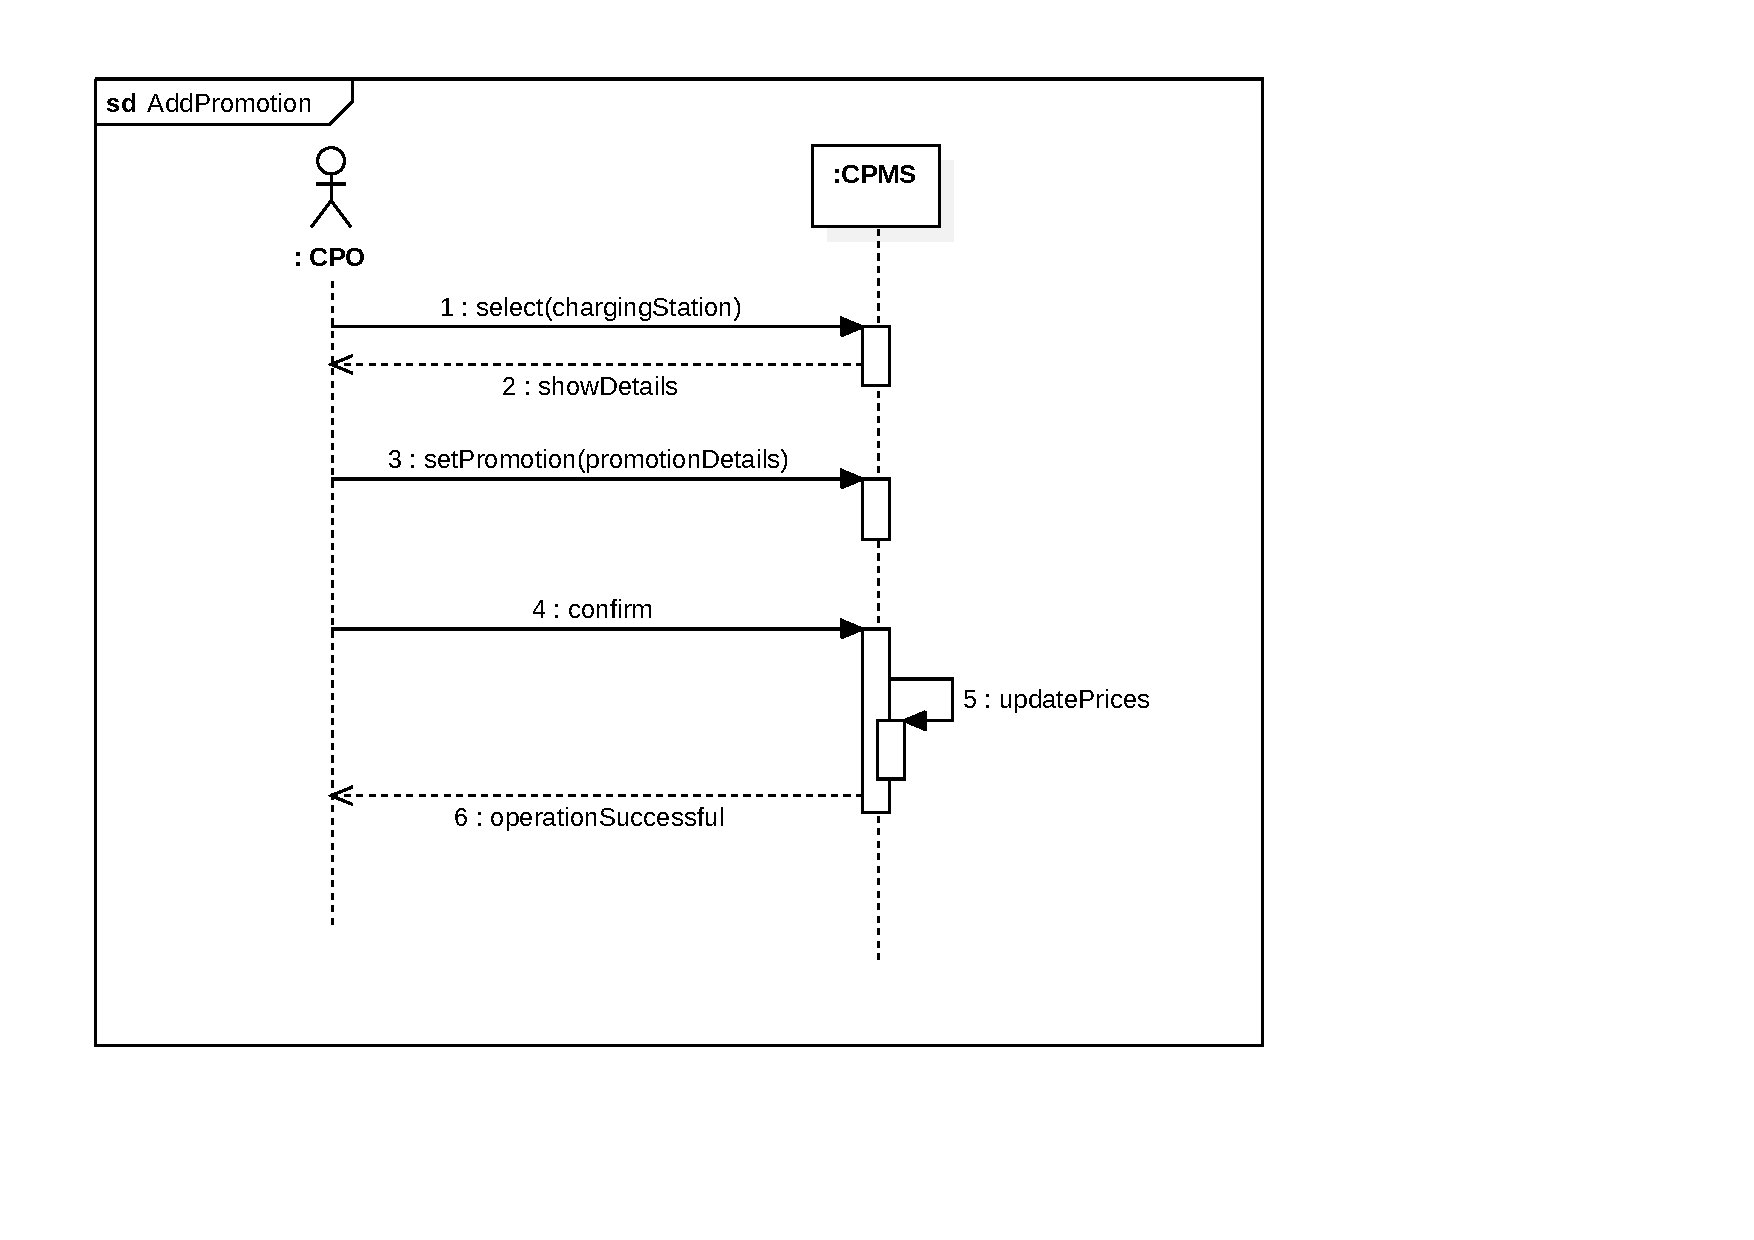
\includegraphics[width=0.8\textwidth, trim={0 3cm 6cm 0}, clip]{Images/cp3/seqDiagrams/AddPromotion.pdf}
%    \caption{AddPromotion sequence diagram}
%\end{figure}

\paragraph{Delete a charging station}
\begin{center}
    \begin{longtable}{p{4cm} p{11cm}}
    \multicolumn{2}{r}{\itshape{continue on the next page}}\\
    \endfoot 
    \\
    \endlastfoot
    \hline
     Use case name &  DeleteChargingStation\\
     \hline
     Actor & CPO \\
     \hline
     Entry condition & The CPO is logged in the web application of the eMall and on the homepage \\
     \hline
     Event flow &   1. On the homepage the eMall shows to the CPO the charging stations associated to the company                   registration and any notification on the stations \newline
                    2. The CPO clicks on a charging station \newline 
                    3. The system shows a form with the details of the station \newline
                    4. The CPO clicks the 'Delete charging station' button \newline
                    5. The system sends a warning message and asks for confirmation, because this is a delicate operation \newline
                    6. The CPO confirms the operation \newline
                    7. The system deletes the charging station from the information related to the company \newline
                    8. The system sends a notification message informing of the success of the operation \newline
                    9. The system reloads the homepage, without the deleted charging station\\
     \hline
     Exit condition &  The CPO closes the page loaded by the system with the updated data of the charging station, returning to the homepage \\
     \hline
     Exceptions &   a. If the CPO doesn't confirm the cancellation of the charging station, after 5 minutes, the                    system reloads the homepage, without applying any change \newline
                    b. If at any time the CPO wants to exit, the application allows it, and no changes will be applied if the procedure wasn't completed \\
     \hline
     Special requirements & After the CPO confirms the operation, the charging station will be deleted from the information related to the company and the homepage will be shown in less than 2 seconds, in order for the application to be perceived as fast\\
     \hline
    \caption{DeleteChargingStation}
    \label{tab:DeleteChargingStation}
    \end{longtable}
\end{center}

\paragraph{Add a charging station}
\begin{center}
    \begin{longtable}{p{4cm} p{11cm}}
    \multicolumn{2}{r}{\itshape{continue on the next page}}\\
    \endfoot 
    \\
    \endlastfoot
    \hline
     Use case name &  AddChargingStation\\
     \hline
     Actor & CPO \\
     \hline
     Entry condition & The CPO is logged in the web application of the eMall and on the homepage \\
     \hline
     Event flow &   1. The CPO selects the button 'Add charging station' \newline
                    2. The system shows a form to fill up with the data related to the new charging station: the code of the station, the position, the charging points, the available sockets, the prices, the batteries of the station and other details for each charging point \newline
                    3. The CPO completes the form and confirms \newline
                    4. The system checks and saves the new data related to the charging station \newline
                    5. The system sends a notification message informing of the success of the operation \newline
                    6. The system loads a page showing the new charging station with the associated information\\
     \hline
     Exit condition &  The CPO closes the page loaded by the system with the updated data of the charging station, returning to the homepage \\
     \hline
     Exceptions &   a. If the CPO doesn't fill up all the mandatory data of the form before submitting it, the eMall                sends a message, which informs what other data are required, and returns to the form that the                   CPO can continue to complete \newline
                    b. If at any time the CPO wants to exit, the application allows it, and no changes will be applied if the procedure wasn't completed \\
     \hline
     Special requirements & After the CPO confirms the operation, the new charging station with the related details is added to the data related to the company, and shown on a new page in less than 2 seconds, in order for the application to be perceived as fast and responsive \\
     \hline
    \caption{AddChargingStation}
    \label{tab:AddChargingStation}
    \end{longtable}
\end{center}

\paragraph{Add a charging point}
\begin{center}
    \begin{longtable}{p{4cm} p{11cm}}
    \multicolumn{2}{r}{\itshape{continue on the next page}}\\
    \endfoot 
    \\
    \endlastfoot
    \hline
     Use case name &  AddChargingPoint\\
     \hline
     Actor & CPO \\
     \hline
     Entry condition & The CPO is logged in the web application of the eMall and on the homepage \\
     \hline
     Event flow & 1. On the homepage the eMall shows to the CPO the charging stations                   associated to the company registration and any notification on the                 stations\newline
                    2. The CPO clicks on a charging station \newline 
                    3. The system shows a form with the details of the charging station \newline
                    4. The CPO clicks the 'Add charging point' button \newline
                    5. The system shows a new form to fill up with the data related to the new charging point: the code of the charging point, the available sockets, the maximum and minimum output capacity and other details \newline
                    6. The CPO completes the form and confirms the operation \newline
                    7. The system checks and saves the new charging point related to the charging station \newline
                    8. The system sends a notification message informing of the success of the operation \newline
                    9. The system loads a page showing the charging stations with the new associated charging point\\
     \hline
     Exit condition &  The CPO closes the page loaded by the system with the updated data of the charging station, returning to the homepage \\
     \hline
     Exceptions &   a. If the CPO doesn't fill up all the mandatory data of the form                    before submitting it, the eMall sends a message, which informs                     what other data are required, and returns to the form, that the                    CPO can continue to complete \newline
                    b. If at any time the CPO wants to exit, the application allows it, and no changes will be applied if the procedure wasn't completed \\
     \hline
     Special requirements & After the CPO confirms the operation, the new charging point of the station, with the related details, is added to the data related to the company, and shown on a new page in less than 2 seconds, in order for the application to be perceived as fast and responsive \\
     \hline
    \caption{AddChargingPoint}
    \label{tab:AddChargingPoint}
    \end{longtable}
\end{center}

\paragraph{Visualize graphical information about the charging stations}
\begin{center}
    \begin{longtable}{p{4cm} p{11cm}}
    \multicolumn{2}{r}{\itshape{continue on the next page}}\\
    \endfoot 
    \\
    \endlastfoot
    \hline
     Use case name &  VisualizeGraphicalInformation\\
     \hline
     Actor & CPO \\
     \hline
     Entry condition & The CPO is logged in the web application of the eMall and on the homepage \\
     \hline
     Event flow &   1. On the homepage the eMall shows to the CPO the charging stations associated to the company                   registration and any notification on the stations \newline
                    2. To see more specific information the CPO click on 'Visualization' button \newline 
                    3. The system shows a list with all the elements that can be visualized in form of a graph regarding the managed charging stations \newline
                    4. The CPO selects the information that is interested in, for example the peak hours and energy requests \newline
                    5. The CPO confirms the operation \newline
                    6. The system processes the chosen data regarding all the stations \newline
                    7. The system loads a new page in which shows some graphical representations of the data \\
     \hline
     Exit condition &  The CPO closes the page loaded by the system with the graphical visualizations of the data of the charging stations, returning to the homepage \\
     \hline
     Exceptions &   a. If the CPO doesn't select anything on the list before submitting it, the eMall sends a                       message which informs that nothing can be visualized, and returns to the homepage \newline
                    b. If at any time the CPO wants to exit, the application allows it, and no changes will be applied if the procedure wasn't completed \\
     \hline
     Special requirements & After the CPO confirms the operation, the graphical visualizations are shown on a new page in less than 2 minutes, in order for the system to have enough time to process a lot of the present data, and show an approximated solution in an acceptable time \\
     \hline
    \caption{VisualizeGraphicalInformation}
    \label{tab:VisualizeGraphicalInformation}
    \end{longtable}
\end{center}

\paragraph{Solve the notification regarding a charging station}
\begin{center}
    \begin{longtable}{p{4cm} p{11cm}}
    \multicolumn{2}{r}{\itshape{continue on the next page}}\\
    \endfoot 
    \\
    \endlastfoot
    \hline
     Use case name &  SolveNotification\\
     \hline
     Actor & CPO \\
     \hline
     Entry condition & The CPO is logged in the web application of the eMall and on the homepage \\
     \hline
     Event flow &   1. On the homepage the eMall shows to the CPO the charging stations associated to the company                   registration and any notification on the stations \newline
                    2. The CPO clicks on a notification \newline 
                    3. The system shows a form with the details of the charging station, with the data related to the notification highlighted in red  \newline
                    4. The CPO clicks on the battery associated to the charging station, that is highlighted in red \newline
                    5. When clicking on a red element, the system shows a notification message, informing the CPO about the problem or the changes undergone to that element of the station \newline
                    6. The CPO solves the notification making some changes on the form \newline
                    7. The CPO confirms the operation \newline
                    8. The system checks and saves the new data related to the charging station \newline
                    9. The system sends a notification message informing of the success of the operation and deletes the notification message present before the operation \newline
                    10. The system loads a page showing the charging station with the new associated information\\
     \hline
     Exit condition &  The CPO closes the page loaded by the system with the updated data of the charging station, returning to the homepage \\
     \hline
     Exceptions &   a. If the CPO doesn't modify anything on the form before submitting it, the eMall sends a                       message which informs that the data have not been modified, and returns to the homepage without                 deleting the notification message from the system \newline
                    b. If the CPO changes the form, but not the details regarding the notification, the eMall will apply the operation, after the submitting of the form, but will maintain the notification message in the system \newline 
                    c. If at any time the CPO wants to exit, the application allows it, and no changes will be applied if the procedure wasn't completed \\
     \hline
     Special requirements & After the CPO confirms the operation, the charging station with the related details is updated and shown on a new page in less than 2 seconds, in order for the application to be perceived as fast and responsive \\
     \hline
    \caption{SolveNotification}
    \label{tab:SolveNotification}
    \end{longtable}
\end{center}

\paragraph{Decide to use the battery}
\begin{center}
    \begin{longtable}{p{4cm} p{11cm}}
    \multicolumn{2}{r}{\itshape{continue on the next page}}\\
    \endfoot 
    \\
    \endlastfoot
    \hline
     Use case name &  UseEnergyFromBattery\\
     \hline
     Actor & CPO \\
     \hline
     Entry condition & The charging station is equipped with a battery \\
     \hline
     Event flow &
        1. CPO selects to change the energy source used by the charging points \newline
        2. CPMS shows to the CPO the list of available energy sources \newline
        3. CPO selects the battery as energy source \newline
        4. The system accepts the instruction and processes the request, checking that the battery is not empty \newline
        5. The system notifies the successful operation
     \\
     \hline
     Exit condition &  The system switches to the battery as energy source for the charging points of the station\\
     \hline
     Exceptions & 
        a. If the battery is empty the system won't allow the user to select it as energy source \newline
        b. If the system can't switch to the battery energy source an error message is sent to the user\\
     \hline
     Special requirements &
        While changing the energy source to battery the system must show to the user the status of the processing in real-time \\
     \hline
    \caption{UseEnergyFromBattery}
    \label{tab:UseEnergyFromBattery}
    \end{longtable}
\end{center}

\clearpage
\paragraph{Decide to store energy in the battery}
\begin{center}
    \begin{longtable}{p{4cm} p{11cm}}
    \multicolumn{2}{r}{\itshape{continue on the next page}}\\
    \endfoot 
    \\
    \endlastfoot
    \hline
     Use case name &  StoreEnergyInBattery\\
     \hline
     Actor & CPO \\
     \hline
     Entry condition & The charging station is equipped with a battery  \\
     \hline
     Event flow & 
        1. CPO selects the battery management section \newline
        2. CPMS shows the status of the battery (remaining charge, in use, functioning) \newline
        3. CPO selects to recharge the battery \newline
        4. CPMS process the request and connects the battery to the station grid \newline
        5. CPMS show information about the charging process
     \\
     \hline
     Exit condition & The battery is charging \\
     \hline
     Exceptions & 
        a. If the battery is already full or malfunctioning then the CPMS will notify the CPO with an error message explaining the reason of the error\\
     \hline
     Special requirements &
        Te system shall process the request in less than 2 seconds\\
     \hline
    \caption{StoreEnergyInBattery}
    \label{tab:StoreEnergyInBattery}
    \end{longtable}
\end{center}
\clearpage